\documentclass{amsart}

\usepackage[utf8]{inputenc}
\usepackage[T2A]{fontenc}
\usepackage[english,russian]{babel}
\usepackage{amsthm,amsmath,amsfonts,amssymb}
\usepackage{fullpage}
\usepackage{eufrak}

%%% Дополнительная работа с математикой
\usepackage{amsfonts,amssymb,amsthm,mathtools} % AMS
\usepackage{amsmath}
\usepackage{icomma}

%% Шрифты
\usepackage{euscript}	 % Шрифт Евклид
\usepackage{mathrsfs} % Красивый матшрифт

%% Свои команды
\DeclareMathOperator{\sgn}{\mathop{sgn}}	% сигнум
\DeclareMathOperator{\cov}{\mathop{cov}}	% ковариация
\DeclareMathOperator{\lb}{\mathop{lb}}	% бинарный логарифм (логарифм по основанию 2)
\DeclareMathOperator{\supp}{\mathop{supp}}	% носитель

\renewcommand{\Im}{\mathop{\mathrm{Im}}\nolimits}	% мнимая часть
\renewcommand{\Re}{\mathop{\mathrm{Re}}\nolimits}	% вещественная часть

\renewcommand{\Prob}{\mathbb P}	% вероятность
\newcommand{\Expect}{\mathbb E}	% математическое ожидание
\renewcommand{\Variance}{\mathbb D}	% дисперсия
\newcommand{\Entropy}{\mathbb H}	% энтропия

%% Перенос знаков в формулах (по Львовскому)
\newcommand*{\hm}[1]{#1\nobreak\discretionary{}
	{\hbox{$\mathsurround=0pt #1$}}{}}

%%% Работа с картинками
\usepackage{graphicx}  % Для вставки рисунков
\graphicspath{{images/}{images2/}}  % папки с картинками
\setlength\fboxsep{3pt} % Отступ рамки \fbox{} от рисунка
\setlength\fboxrule{1pt} % Толщина линий рамки \fbox{}
\usepackage{wrapfig} % Обтекание рисунков и таблиц текстом
\RequirePackage{caption}
\DeclareCaptionLabelSeparator{defffis}{ -- }
\captionsetup{justification=centering,labelsep=defffis}

\renewcommand{\qedsymbol}{}

%%% Работа с таблицами
\usepackage{array,tabularx,tabulary,booktabs} % Дополнительная работа с таблицами
\usepackage{longtable}  % Длинные таблицы
\usepackage{multirow} % Слияние строк в таблице

\newtheorem{problem}{Задание}

\begin{document}

	\newcommand{\problemset}[1]{
		\begin{center}
			\Large #1
		\end{center}
	}

	\begin{tabbing}
	\hspace{11cm} \= Студент: \= Коротков Фёдор \\ % не забудьте исправить, студент Вы или студентка :)
																									% (а то некоторые забывают)
	\> Группа: \> 2362 \\  % Здесь меняете № группы
	\> Вариант: \> QG \\    % А здесь меняете № варианта
	\> Дата: \> \today     % А вот здесь ничего не меняем!!!
\end{tabbing}
\hrule
\vspace{1cm}  % в данном файле меняем только Пол, Фамилию Имя, № группы и № варианта
	\problemset{Комбинаторика и теория графов}
\problemset{Индивидуальное домашнее задание №1}	% поменяйте номер ИДЗ

\renewcommand*{\proofname}{Решение}
%%%%%%%%%%%%%% ЗАДАНИЕ №1 %%%%%%%%%%%%%%
%% Условие задания №1
\begin{problem}
	Дано множество М = $\{19, 33, 69, 72, 77, 91, 96, 97\}$
    и следующие бинарные отношения на нем:
    \begin{itemize}
    
    \item $F_1(x,y) = 1 \Leftrightarrow \exists z \in M : (x - z)(y - z) < 0;$

    \item $F_2(x, y) = 1 \Leftrightarrow x \geq y$ поразрядно;

    \item $F_3(x, y) = 1 \Leftrightarrow [\frac{x}{5}] = [\frac{y}{5}]$;

    \item $F_4(x,y) = 1 \Leftrightarrow x^2 - y^3$ нечетно;

    \item $F_5(x, y) = 1 \Leftrightarrow |x-y| < 10$.
    \end{itemize}
    Для каждого из отношений:

    \begin{enumerate}

    \item[1.] Проверить, является ли бинарное отношение (далее -  б.о.) - рефлексивным, арефлексивным, симметричным, антисимметричным, асимметричным, транзитивным.
    \item[2.] Построить матрицы и графы этих б.о.

    \item[3.] Определить, являются ли эти б.о. отношениями эквивалентности, частичного порядка, линейного порядка, строгого порядка).

    \item[4.] Для отношений эквивалентности построить классы эквивалентности.

    \item[5.] Для отношений частичного порядка применить алгоритм топологической сортировки и получить отношение линейного порядка.

    \item[6.] Для нетранзитивных отношений построить транзитивное замыкание, используя алгоритм Уоршелла.
    \end{enumerate}
\end{problem}

%% Решение задания №1
\pagebreak
\begin{proof} \textbf{Бинарное отношение $F_1$}\\
Отношение $F_1$ можно переформулирвоать, как $\exists z \in M: x < z < y \text{ или } y < z < x$
\\ \\
Построим матрицу смежности для б.о. $F_1$
$$ \left( \begin{array}{cccccccc}
		   0 &0 &1 &1 &1 &1 &1 &1 
        \\0 &0 &0 &1 &1 &1 &1 &1
        \\1 &0 &0 &0 &1 &1 &1 &1
        \\1 &1 &0 &0 &0 &1 &1 &1
        \\1 &1 &1 &0 &0 &0 &1 &1
        \\1 &1 &1 &1 &0 &0 &0 &1
        \\1 &1 &1 &1 &1 &0 &0 &0
        \\1 &1 &1 &1 &1 &1 &0 &0 \end{array} \right) $$\\
Из матрицы смежности видно, что бинарное отношение $F_1$ является арефлексивным, т.к. элементы матрицы смежности на главной диагонали не равны единице, и симметричным, т.к. относительно главной диагонали матрица зеркальна.
\\ \\
Построим граф для б.о. $F_1$:

\tikz {
        \path
(4.0, 8.0) node[state] (1) {19}
(6.83, 6.83) node[state] (2) {33}
(8.0, 4.0) node[state] (3) {69}
(6.83, 1.17) node[state] (4) {72}
(4.0, 0.0) node[state] (5) {77}
(1.17, 1.17) node[state] (6) {91}
(0.0, 4.0) node[state] (7) {96}
(1.17, 6.83) node[state] (8) {97};
\draw (1) -- (3);
\draw (1) -- (4);
\draw (1) -- (5);
\draw (1) -- (6);
\draw (1) -- (7);
\draw (1) -- (8);
\draw (2) -- (4);
\draw (2) -- (5);
\draw (2) -- (6);
\draw (2) -- (7);
\draw (2) -- (8);
\draw (3) -- (5);
\draw (3) -- (6);
\draw (3) -- (7);
\draw (3) -- (8);
\draw (4) -- (6);
\draw (4) -- (7);
\draw (4) -- (8);
\draw (5) -- (7);
\draw (5) -- (8);
\draw (6) -- (8);
}\\
Бинарное отношение не является транзитивным, т.к., например, между вершинами 96 и 97 есть путь длины 2, но нет пути длины 1.
\ \
Отношение $F_1$:
\begin{itemize}
    \item Арефлексивное
    \item Симметричное
    \item Не транзитивное 
\end{itemize}
\ \
Для построения транзитивного замыкания применим алгоритм Уоршелла:
$$ \left( \begin{array}{cccccccc}
		   0 &0 &1 &1 &1 &1 &1 &1 
        \\0 &0 &0 &1 &1 &1 &1 &1
        \\1 &0 &0 &0 &1 &1 &1 &1
        \\1 &1 &0 &0 &0 &1 &1 &1
        \\1 &1 &1 &0 &0 &0 &1 &1
        \\1 &1 &1 &1 &0 &0 &0 &1
        \\1 &1 &1 &1 &1 &0 &0 &0
        \\1 &1 &1 &1 &1 &1 &0 &0 \end{array} \right) \Rightarrow
    \left( \begin{array}{cccccccc}
		   0 &0 &1 &1 &1 &1 &1 &1 
        \\0 &0 &0 &1 &1 &1 &1 &1
        \\1 &0 &\textcolor{red}{1} &\textcolor{red}{1} &1 &1 &1 &1
        \\1 &1 &\textcolor{red}{1} &\textcolor{red}{1} &\textcolor{red}{1} &1 &1 &1
        \\1 &1 &1 &\textcolor{red}{1} &\textcolor{red}{1} &\textcolor{red}{1} &1 &1
        \\1 &1 &1 &1 &\textcolor{red}{1} &\textcolor{red}{1} &\textcolor{red}{1} &1
        \\1 &1 &1 &1 &1 &\textcolor{red}{1} &\textcolor{red}{1} &\textcolor{red}{1}
        \\1 &1 &1 &1 &1 &1 &\textcolor{red}{1} &\textcolor{red}{1} \end{array} \right) \Rightarrow
    \left( \begin{array}{cccccccc}
		   \textcolor{red}{1} &\textcolor{red}{1} &1 &1 &1 &1 &1 &1 
        \\\textcolor{red}{1} &\textcolor{red}{1} &\textcolor{red}{1} &1 &1 &1 &1 &1
        \\1 &\textcolor{red}{1} &1 &1 &1 &1 &1 &1
        \\1 &1 &1 &1 &1 &1 &1 &1
        \\1 &1 &1 &1 &1 &1 &1 &1
        \\1 &1 &1 &1 &1 &1 &1 &1
        \\1 &1 &1 &1 &1 &1 &1 &1
        \\1 &1 &1 &1 &1 &1 &1 &1 \end{array} \right)    
        $$
\end{proof}

\pagebreak
\begin{proof} \textbf{Бинарное отношение $F_2$}\\
Построим матрицу смежности для б.о. $F_2$
$$ \left( \begin{array}{cccccccc}
		   1 &0 &0 &0 &0 &0 &0 &0 
        \\0 &1 &0 &0 &0 &0 &0 &0
        \\1 &1 &1 &0 &0 &0 &0 &0
        \\0 &0 &0 &1 &0 &0 &0 &0
        \\0 &1 &0 &1 &1 &0 &0 &0
        \\0 &0 &0 &0 &0 &1 &0 &0
        \\0 &1 &0 &1 &0 &1 &1 &0
        \\0 &1 &0 &1 &1 &1 &1 &1 \end{array} \right) $$\\
Бинарное отношение $F_2$ рефлексивное, т.к все элементы матрицы смежности на главной диагонали равны единице, и антисимметричное, т.к. выше главное диагонали в матрице находятся только 0.

\tikz {
	\path
(4.0, 8.0) node[state] (1) {19}
(6.83, 6.83) node[state] (2) {33}
(8.0, 4.0) node[state] (3) {69}
(6.83, 1.17) node[state] (4) {72}
(4.0, 0.0) node[state] (5) {77}
(1.17, 1.17) node[state] (6) {91}
(0.0, 4.0) node[state] (7) {96}
(1.17, 6.83) node[state] (8) {97};
\draw[->] (1) to [out=45.0,in=90.0,looseness=5] (1);
\draw[->] (2) to [out=0.0,in=45.0,looseness=5] (2);
\draw[->] (3) -- (1);
\draw[->] (3) -- (2);
\draw[->] (3) to [out=-45.0,in=0.0,looseness=5] (3);
\draw[->] (4) to [out=-90.0,in=-45.0,looseness=5] (4);
\draw[->] (5) -- (2);
\draw[->] (5) -- (4);
\draw[->] (5) to [out=-135.0,in=-90.0,looseness=5] (5);
\draw[->] (6) to [out=-180.0,in=-135.0,looseness=5] (6);
\draw[->] (7) -- (2);
\draw[->] (7) -- (4);
\draw[->] (7) -- (6);
\draw[->] (7) to [out=-225.0,in=-180.0,looseness=5] (7);
\draw[->] (8) -- (2);
\draw[->] (8) -- (4);
\draw[->] (8) -- (5);
\draw[->] (8) -- (6);
\draw[->] (8) -- (7);
\draw[->] (8) to [out=-270.0,in=-225.0,looseness=5] (8);
}\\
Бинарное отношение $F_2$ транзитивно, т.к. для любых вершин, между котрыми есть путь длины 2 найдется и путь длины 1.
\\ \\
Отношение $F_2$:
\begin{itemize}
    \item Рефлексивное
    \item Антисимметричное
    \item Транзитивное
\end{itemize}
Соответственно, оно является отношением частичного порядка (не линейный порядок, т.к. на графе не между всеми вершинами есть ребро).
\\ \\
Граф после применения топологической сортировки для дополнения отношения $F_2$ до отношения линейного порядка будет выглядеть следующим образом (если в качестве начальной вершины каждый раз принимать вершину с наименьшим значением из множества ещё не пройденных вершин, то с возрастанием номера вершины, её номер будет наоборот убывать):

\tikz {
	\path
(4.0, 8.0) node[state] (1) {19}
(6.83, 6.83) node[state] (2) {33}
(8.0, 4.0) node[state] (3) {69}
(6.83, 1.17) node[state] (4) {72}
(4.0, 0.0) node[state] (5) {77}
(1.17, 1.17) node[state] (6) {91}
(0.0, 4.0) node[state] (7) {96}
(1.17, 6.83) node[state] (8) {97};
\draw[->] (1) to [out=45.0,in=90.0,looseness=5] (1);
\draw[->] (2) to [out=0.0,in=45.0,looseness=5] (2);
\draw[->] (3) -- (1);
\draw[->] (3) -- (2);
\draw[->] (3) to [out=-45.0,in=0.0,looseness=5] (3);
\draw[->] (4) to [out=-90.0,in=-45.0,looseness=5] (4);
\draw[->] (5) -- (2);
\draw[->] (5) -- (4);
\draw[->] (5) to [out=-135.0,in=-90.0,looseness=5] (5);
\draw[->] (6) to [out=-180.0,in=-135.0,looseness=5] (6);
\draw[->] (7) -- (2);
\draw[->] (7) -- (4);
\draw[->] (7) -- (6);
\draw[->] (7) to [out=-225.0,in=-180.0,looseness=5] (7);
\draw[->] (8) -- (2);
\draw[->] (8) -- (4);
\draw[->] (8) -- (5);
\draw[->] (8) -- (6);
\draw[->] (8) -- (7);
\draw[->] (8) to [out=-270.0,in=-225.0,looseness=5] (8);
\draw[->][densely dotted] (8) -- (1);
\draw[->][densely dotted] (8) -- (3);
\draw[->][densely dotted] (7) -- (1);
\draw[->][densely dotted] (7) -- (3);
\draw[->][densely dotted] (7) -- (5);
\draw[->][densely dotted] (6) -- (1);
\draw[->][densely dotted] (6) -- (2);
\draw[->][densely dotted] (6) -- (3);
\draw[->][densely dotted] (6) -- (4);
\draw[->][densely dotted] (6) -- (5);
\draw[->][densely dotted] (5) -- (1);
\draw[->][densely dotted] (5) -- (3);
\draw[->][densely dotted] (4) -- (1);
\draw[->][densely dotted] (4) -- (2);
\draw[->][densely dotted] (4) -- (3);
\draw[->][densely dotted] (2) -- (1);
}\\
А матрица линейного отношения $F_2$, дополненного до отношения линецйного порядка, будет соответствовать данной (все нули под главной диагональю становятся единицами):
$$ \left( \begin{array}{cccccccc}
		   1 &0 &0 &0 &0 &0 &0 &0 
        \\1 &1 &0 &0 &0 &0 &0 &0
        \\1 &1 &1 &0 &0 &0 &0 &0
        \\1 &1 &1 &1 &0 &0 &0 &0
        \\1 &1 &1 &1 &1 &0 &0 &0
        \\1 &1 &1 &1 &1 &1 &0 &0
        \\1 &1 &1 &1 &1 &1 &1 &0
        \\1 &1 &1 &1 &1 &1 &1 &1 \end{array} \right) $$
\end{proof}

\pagebreak
\begin{proof} \textbf{Бинарное отношение $F_3$}\\
Построим матрицу смежности для б.о. $F_3$
$$ \left( \begin{array}{cccccccc}
		   1 &0 &0 &0 &0 &0 &0 &0 
        \\0 &1 &0 &0 &0 &0 &0 &0
        \\0 &0 &1 &0 &0 &0 &0 &0
        \\0 &0 &0 &1 &0 &0 &0 &0
        \\0 &0 &0 &0 &1 &0 &0 &0
        \\0 &0 &0 &0 &0 &1 &0 &0
        \\0 &0 &0 &0 &0 &0 &1 &1
        \\0 &0 &0 &0 &0 &0 &1 &1 \end{array} \right) $$
Бинарное отношение $F_3$ рефлексивное, т.к все элементы матрицы смежности на главной диагонали равны единице, и симметричное, т.к. матрица зеркальна относительно главной диагонали.

\tikz {
	\path
(4.0, 8.0) node[state] (1) {19}
(6.83, 6.83) node[state] (2) {33}
(8.0, 4.0) node[state] (3) {69}
(6.83, 1.17) node[state] (4) {72}
(4.0, 0.0) node[state] (5) {77}
(1.17, 1.17) node[state] (6) {91}
(0.0, 4.0) node[state] (7) {96}
(1.17, 6.83) node[state] (8) {97};
\draw[->] (1) to [out=45.0,in=90.0,looseness=5] (1);
\draw[->] (2) to [out=0.0,in=45.0,looseness=5] (2);
\draw[->] (3) to [out=-45.0,in=0.0,looseness=5] (3);
\draw[->] (4) to [out=-90.0,in=-45.0,looseness=5] (4);
\draw[->] (5) to [out=-135.0,in=-90.0,looseness=5] (5);
\draw[->] (6) to [out=-180.0,in=-135.0,looseness=5] (6);
\draw[->] (7) to [out=-225.0,in=-180.0,looseness=5] (7);
\draw (7) -- (8);
\draw[->] (8) to [out=-270.0,in=-225.0,looseness=5] (8);
}\\
Бинарное отношение $F_3$ транзитивно, т.к. на графе отсутствуют пути длины 2.
\\ \\
Отношение $F_3$:
\begin{itemize}
    \item Рефлексивное
    \item Симметричное
    \item Транзитивное
\end{itemize}
Соответственно, оно является отношением эквивалентности.
Множество M разбивается на классы эквивалентности по целой части при делении на 5. А именно:
\begin{itemize}
    \item $\{19\}$ - целая часть = 2
    \item $\{33\}$ - целая часть = 6
    \item $\{69\}$ - целая часть = 13
    \item $\{72\}$ - целая часть = 14
    \item $\{77\}$ - целая часть = 15
    \item $\{91\}$ - целая часть = 18
    \item $\{96, 97\}$ - целая часть = 19
\end{itemize}
\end{proof}

% \pagebreak
\begin{proof} \textbf{Бинарное отношение $F_4$}\\
Построим матрицу смежности для б.о. $F_4$
$$ \left( \begin{array}{cccccccc}
		   0 &0 &0 &1 &0 &0 &1 &0 
        \\0 &0 &0 &1 &0 &0 &1 &0 
        \\0 &0 &0 &1 &0 &0 &1 &0 
        \\1 &1 &1 &0 &1 &1 &0 &1 
        \\0 &0 &0 &1 &0 &0 &1 &0 
        \\0 &0 &0 &1 &0 &0 &1 &0 
        \\1 &1 &1 &0 &1 &1 &0 &1 
        \\0 &0 &0 &1 &0 &0 &1 &0 \end{array} \right) $$
Бинарное отношение $F_4$ арефлексивное, т.к. элементы матрицы смежности на главной диагонали не равны единице, и  симметричное, т.к. матрица зеркальна относительно главной диагонали.


\tikz {
	\path
(4.0, 8.0) node[state] (1) {19}
(6.83, 6.83) node[state] (2) {33}
(8.0, 4.0) node[state] (3) {69}
(6.83, 1.17) node[state] (4) {72}
(4.0, 0.0) node[state] (5) {77}
(1.17, 1.17) node[state] (6) {91}
(0.0, 4.0) node[state] (7) {96}
(1.17, 6.83) node[state] (8) {97};
\draw (1) -- (4);
\draw (1) -- (7);
\draw (2) -- (4);
\draw (2) -- (7);
\draw (3) -- (4);
\draw (3) -- (7);
\draw (4) -- (5);
\draw (4) -- (6);
\draw (4) -- (8);
\draw (5) -- (7);
\draw (6) -- (7);
\draw (7) -- (8);
}\\
Бинарное отношение $F_4$ не транзитивно. Например, между вершинами 96 и 72 есть несколько путей длины 2, но нет ни одного пути длиной 1.
\\ \\
Отношение $F_4$:
\begin{itemize}
    \item Арефлексивное
    \item Симметричное
    \item Не транзитивное
\end{itemize}

Для построения транзитивного замыкания применим алгоритм Уоршелла:
$$ \left( \begin{array}{cccccccc}
		   0 &0 &0 &1 &0 &0 &1 &0 
        \\0 &0 &0 &1 &0 &0 &1 &0 
        \\0 &0 &0 &1 &0 &0 &1 &0 
        \\1 &1 &1 &0 &1 &1 &0 &1 
        \\0 &0 &0 &1 &0 &0 &1 &0 
        \\0 &0 &0 &1 &0 &0 &1 &0 
        \\1 &1 &1 &0 &1 &1 &0 &1 
        \\0 &0 &0 &1 &0 &0 &1 &0 \end{array} \right) \Rightarrow
    \left( \begin{array}{cccccccc}
		   0 &0 &0 &1 &0 &0 &1 &0 
        \\0 &0 &0 &1 &0 &0 &1 &0 
        \\0 &0 &0 &1 &0 &0 &1 &0 
        \\1 &1 &1 &\textcolor{red}{1} &1 &1 &\textcolor{red}{1} &1 
        \\0 &0 &0 &1 &0 &0 &1 &0 
        \\0 &0 &0 &1 &0 &0 &1 &0 
        \\1 &1 &1 &\textcolor{red}{1} &1 &1 &\textcolor{red}{1} &1 
        \\0 &0 &0 &1 &0 &0 &1 &0 \end{array} \right) \Rightarrow
    \left( \begin{array}{cccccccc}
		   \textcolor{red}{1} &\textcolor{red}{1} &\textcolor{red}{1} &1 &\textcolor{red}{1} &\textcolor{red}{1} &1 &\textcolor{red}{1} 
        \\\textcolor{red}{1} &\textcolor{red}{1} &\textcolor{red}{1} &1 &\textcolor{red}{1} &\textcolor{red}{1} &1 &\textcolor{red}{1} 
        \\\textcolor{red}{1} &\textcolor{red}{1} &\textcolor{red}{1} &1 &\textcolor{red}{1} &\textcolor{red}{1} &1 &\textcolor{red}{1} 
        \\1 &1 &1 &1 &1 &1 &1 &1 
        \\\textcolor{red}{1} &\textcolor{red}{1} &\textcolor{red}{1} &1 &\textcolor{red}{1} &\textcolor{red}{1} &1 &\textcolor{red}{1} 
        \\\textcolor{red}{1} &\textcolor{red}{1} &\textcolor{red}{1} &1 &\textcolor{red}{1} &\textcolor{red}{1} &1 &\textcolor{red}{1} 
        \\1 &1 &1 &1 &1 &1 &1 &1 
        \\\textcolor{red}{1} &\textcolor{red}{1} &\textcolor{red}{1} &1 &\textcolor{red}{1} &\textcolor{red}{1} &1 &\textcolor{red}{1} \end{array} \right)    
        $$
\end{proof}

\pagebreak
\begin{proof} \textbf{Бинарное отношение $F_5$}\\
Построим матрицу смежности для б.о. $F_5$\\
$$ \left( \begin{array}{cccccccc}
          1 &0 &0 &0 &0 &0 &0 &0
        \\0 &1 &0 &0 &0 &0 &0 &0
        \\0 &0 &1 &1 &1 &0 &0 &0
        \\0 &0 &1 &1 &1 &0 &0 &0
        \\0 &0 &1 &1 &1 &0 &0 &0
        \\0 &0 &0 &0 &0 &1 &1 &1
        \\0 &0 &0 &0 &0 &1 &1 &1
        \\0 &0 &0 &0 &0 &1 &1 &1 \end{array} \right) $$
Бинарное отношение $F_5$ рефлексивное, т.к все элементы матрицы смежности на главной диагонали равны единице, и симметричное, т.к. матрица зеркальна относительно главной диагонали.


\tikz {
	\path
(4.0, 8.0) node[state] (1) {19}
(6.83, 6.83) node[state] (2) {33}
(8.0, 4.0) node[state] (3) {69}
(6.83, 1.17) node[state] (4) {72}
(4.0, 0.0) node[state] (5) {77}
(1.17, 1.17) node[state] (6) {91}
(0.0, 4.0) node[state] (7) {96}
(1.17, 6.83) node[state] (8) {97};
\draw[->] (1) to [out=45.0,in=90.0,looseness=5] (1);
\draw[->] (2) to [out=0.0,in=45.0,looseness=5] (2);
\draw[->] (3) to [out=-45.0,in=0.0,looseness=5] (3);
\draw (3) -- (4);
\draw (3) -- (5);
\draw[->] (4) to [out=-90.0,in=-45.0,looseness=5] (4);
\draw (4) -- (5);
\draw[->] (5) to [out=-135.0,in=-90.0,looseness=5] (5);
\draw[->] (6) to [out=-180.0,in=-135.0,looseness=5] (6);
\draw (6) -- (7);
\draw (6) -- (8);
\draw[->] (7) to [out=-225.0,in=-180.0,looseness=5] (7);
\draw (7) -- (8);
\draw[->] (8) to [out=-270.0,in=-225.0,looseness=5] (8);
}\\
Бинарное отношение $F_5$ транзитивно, т.к. для всех вершин, между которыми есть путь длины 2, есть и путь длины 1.
\\ \\
Отношение $F_5$:
\begin{itemize}
    \item Рефлексивное
    \item Симметричное
    \item Транзитивное
\end{itemize}
Соответственно оно является отношением эквивалентности.
\\ \\
Множество M будет разбито на классы эквивалентности по разности между элементами < 10, а именно:
\begin{itemize}
    \item $\{19\}$ - нет больше элементов, разность с которыми будет < 10
    \item $\{33\}$ - нет больше элементов, разность с которыми будет < 10
    \item $\{69, 72, 77\}$ - разность между любыми 2-мя элементами < 10
    \item $\{91, 96, 97\}$ - разность между любыми 2-мя элементами < 10
\end{itemize}
\end{proof}





        
 
 
    \problemset{Комбинаторика и теория графов}
\problemset{Индивидуальное домашнее задание №2}	% поменяйте номер ИДЗ

\renewcommand*{\proofname}{Решение}

\begin{problem}
Является ли граф а) эйлеровым, полуэйлеровым?
б) гамильтоновым, полугамильтоновым? в) двудольным? г)
вершинно-двусвязным; д) рёберно-двусвязным е) постройте
дерево блоков и точек сочленения. \\
\usetikzlibrary{graphs,automata,positioning}
\tikz {
	\path
(2, 0) node (A) {A}
(4, 0) node (B) {B}
(0, -2) node (C) {C}
(2, -2) node (D) {D}
(4, -2) node (E) {E}
(6, -2) node (F) {F}
(0, -4) node (G) {G}
(2, -4) node (H) {H}
(4, -4) node (I) {I}
(6, -4) node (J) {J}
(2, -6) node (K) {K}
(4, -6) node (L) {L};
\draw (A) -- (B);
\draw (A) -- (E);
\draw (B) -- (D);
\draw (C) -- (D);
\draw (C) -- (G);
\draw (D) -- (E);
\draw (D) -- (H);
\draw (E) -- (I);
\draw (F) -- (I);
\draw (F) -- (J);
\draw (G) -- (D);
\draw (H) -- (I);
\draw (I) -- (L);
\draw (K) -- (H);
\draw (K) -- (L);
\draw (L) -- (L);
}
\end{problem}

\begin{proof} $ $
    \begin{enumerate}[label=\asbuk*), ref=\asbuk*]
        \item \textbf{эйлеровым, полуэйлеровым?\\}
        Граф не является ни эйлеровым, ни полуэйлеровым, так как в графе есть вершины с нечётными степенями, и их больше двух (D, E, H, J).
        \item \textbf{гамильтоновым, полугамильтоновым?\\}
        В графе есть лист J, следовательно, он не является гамильтоновым. Так как между шарнирами D и I нет простого пусти, содержащего вершины A, B, E, H, K, L, то граф не является полугамильтоновым.
        \item \textbf{двудольным?\\}
\usetikzlibrary{graphs,automata,positioning}
\tikz {
	\path
(1, 0) node (A) {A$^*$}
(2, 0) node (B) {B$^\#$}
(0, -1) node (C) {C$^\#$}
(1, -1) node (D) {D$^*$}
(2, -1) node (E) {E$^\#$}
(3, -1) node (F) {F$^\#$}
(0, -2) node (G) {G$^\#$}
(1, -2) node (H) {H$^\#$}
(2, -2) node (I) {I$^*$}
(3, -2) node (J) {J$^*$}
(1, -3) node (K) {K$^*$}
(2, -3) node (L) {L$^\#$};
\draw (A) -- (B);
\draw (A) -- (E);
\draw (B) -- (D);
\draw (C) -- (D);
\draw (C) -- (G);
\draw (D) -- (E);
\draw (D) -- (H);
\draw (E) -- (I);
\draw (F) -- (I);
\draw (F) -- (J);
\draw (G) -- (D);
\draw (H) -- (I);
\draw (I) -- (L);
\draw (K) -- (H);
\draw (K) -- (L);
\draw (L) -- (L);
}\\
    Так как при раскрашивании смежные вершины C и G оказались одного цвета, граф не является двудольным.
    \item \textbf{вершинно-двусвязным?\\}
    Так как в графе присутствуют шарниры (D, F, I), то граф не может быть вершинно-двусвязным. 
    \item \textbf{рёберно-двусвязным?\\}
    Так как в графе есть мосты (FI, FJ), то граф не является рёберно-двусвязным.
    \item \textbf{постройте
дерево блоков и точек сочленения.\\}
\usetikzlibrary{graphs,automata,positioning}
\tikz {
	\path
(0, 0) node[white, circle,fill=black] (CG) {CG}
(2, 0) node[circle,fill=red] (D) {D}
(10, 0) node[circle,fill=red] (F) {F}
(4, -2) node[white, circle,fill=black] (ABEHKL) {ABEHKL}
(8, -2) node[white, circle,fill=black] (IF) {IF}
(10, -2) node[white, circle,fill=black] (J) {J}
(6, -4) node[circle,fill=red] (I) {I};
\draw (CG) -- (D);
\draw (D) -- (ABEHKL);
\draw (ABEHKL) -- (I);
\draw (F) -- (IF);
\draw (F) -- (J);
\draw (IF) -- (I);
}
    \end{enumerate}
\end{proof}

\begin{problem}
\end{problem}

\begin{proof} $ $
\end{proof}

\begin{problem}
\end{problem}

\begin{proof} $ $
\end{proof}

\begin{problem}
а) Постройте код Прюфера для данного дерева:\\
\usetikzlibrary{graphs,automata,positioning}
\tikz {
	\path
(0, 0) node (1) {1}
(2, 0) node (2) {2}
(4, 0) node (3) {3}
(6, 0) node (4) {4}
(8, 0) node (5) {5}
(10, 0) node (6) {6}
(0, -2) node (7) {7}
(2, -2) node (8) {8}
(4, -2) node (9) {9}
(6, -2) node (10) {10}
(8, -2) node (11) {11};
\draw (1) -- (2);
\draw (2) -- (3);
\draw (3) -- (7);
\draw (4) -- (7);
\draw (5) -- (7);
\draw (6) -- (11);
\draw (8) -- (5);
\draw (9) -- (10);
\draw (10) -- (11);
\draw (11) -- (5);
} \\
б) Постройте дерево по коду Прюфера: 3 9 4 9 10 1 1 9 10.
\end{problem}

\begin{proof} $ $
    \begin{enumerate}[label=\asbuk*), ref=\asbuk*]
        \item \textbf{Построим код Прюфера\\}
        2 3 7 7 11 5 5 11 10 11
        \item \textbf{Построим дерево по коду\\}
        Код: 3 9 4 9 10 1 1 9 10 \\
        Порядок: 2 3 5 4 6 7 8 1 9\\
        \usetikzlibrary{graphs,automata,positioning}
\tikz {
	\path
(0, 0) node (2) {2}
(2, 0) node (3) {3}
(4, 0) node (9) {9}
(6, 0) node (10) {10}
(8, 0) node (6) {6}
(0, -2) node (5) {5}
(2, -2) node (4) {4}
(4, -2) node (7) {7}
(6, -2) node (1) {1}
(8, -2) node (8) {8};
\draw (1) -- (7);
\draw (1) -- (8);
\draw (2) -- (3);
\draw (3) -- (9);
\draw (4) -- (5);
\draw (4) -- (9);
\draw (6) -- (10);
\draw (9) -- (1);
\draw (9) -- (10);
}
    \end{enumerate}
\end{proof}

\begin{problem}
\end{problem}

\begin{proof} $ $
\end{proof}

\begin{problem}
\end{problem}

\begin{proof} $ $
\end{proof}

\begin{problem}
\end{problem}

\begin{proof} $ $
\end{proof}

\begin{problem}
Найдите наибольшее паросочетание в двудольном графе, заданном набором рёбер: (a, $\beta$) (a, $\eta$) (b, $\beta$) (b, $\varepsilon$) (c, $\alpha$)
(c, $\zeta$) (d, $\varepsilon$) (e, $\zeta$) (e, $\eta$) (e, $\theta$) (f, $\gamma$) (f, $\delta$) (f, $\eta$) (g, $\zeta$) (h, $\beta$) (h, $\gamma$)
\end{problem}

\begin{proof} $\\$
\usetikzlibrary{graphs,automata,positioning}
\tikz {
	\path
(0, -7) node (S) {S}
(2, 0) node (a) {a}
(8, 0) node (1) {$\alpha$}
(2, -2) node (b) {b}
(8, -2) node (2) {$\beta$}
(2, -4) node (c) {c}
(8, -4) node (3) {$\eta$}
(2, -6) node (d) {d}
(8, -6) node (4) {$\varepsilon$}
(2, -8) node (e) {e}
(8, -8) node (5) {$\zeta$}
(2, -10) node (f) {f}
(8, -10) node (6) {$\theta$}
(2, -12) node (g) {g}
(8, -12) node (7) {$\gamma$}
(2, -14) node (h) {h}
(8, -14) node (8) {$\delta$}
(10, -7) node (F) {F};
\draw[->] (a) -- (2);
\draw[<-][very thick] (a) -- (3);
\draw[<-][very thick] (b) -- (2);
\draw[->] (b) -- (4);
\draw[<-][very thick] (c) -- (1);
\draw[->] (c) -- (5);
\draw[<-][very thick] (d) -- (4);
\draw[->] (e) -- (5);
\draw[->] (e) -- (3);
\draw[<-][very thick] (e) -- (6);
\draw[->] (f) -- (7);
\draw[<-][very thick] (f) -- (8);
\draw[->] (f) -- (3);
\draw[<-][very thick] (g) -- (5);
\draw[->] (h) -- (2);
\draw[<-][very thick] (h) -- (7);
}
\\ Ответ: (a, $\eta$) (b, $\beta$) (c, $\alpha$)
(d, $\varepsilon$) (e, $\theta$) (f, $\delta$)  (g, $\zeta$) (h, $\gamma$)
\end{proof}
    %%%%%%%%%%%%%% ЗАДАНИЕ №1 %%%%%%%%%%%%%%
%% Условие задания №1
\begin{problem}
    
    М=\{33, 97, 69, 71, 42, 49, 51, 59\}\newline
	Бинарное отношение задано выражением: \newline
   $$ F_{1}(x,y)=1\Leftrightarrow\newline$$
 \newline
 Проверить, является ли бинарное отношение (далее -- б.о.) -- рефлексивным, арефлексивным, симметричным, антисимметричным, асимметричным, транзитивным.
\end{problem}

%% Решение задания №1
\begin{proof}
    Для удобства расположим числа, входящие в мн-во М в порядке возрастания и построим матрицу для данного бинарного отношения:
	$$ \left( \begin{array}{c c c c c c c c } 
 
 1 & 0 & 0 & 0 & 0 & 0 & 0 & 0 \\ 

 0 & 1 & 0 & 0 & 0 & 0 & 0 & 0 \\

 0 & 0 & 1 & 0 & 0 & 0 & 0 & 0 \\
 
 0 & 0 & 0 & 1 & 0 & 0 & 0 & 0 \\
 
 0 & 0 & 0 & 0 & 1 & 0 & 0 & 0 \\
 
 0 & 0 & 0 & 0 & 0 & 1 & 0 & 0 \\
 
 0 & 0 & 0 & 0 & 0 & 0 & 1 & 0 \\
 
 0 & 0 & 0 & 0 & 0 & 0 & 0 & 1 \end {array} \right) $$
 Б.о. рефлексивно, тк на главной диагонали матрицы все 1.
    \newline
     Б.о. симметрично, тк матрица симметрична относительно главной диагонали.
    \newline
     Б.о. антисимметрично, тк выполняется условие $x \ge y$ \wedge $y \ge x$ \Rightarrow $x = y$.
    \newline
    Б.о. транзитивно, тк при возведении матрицы в квадрат не появляются новые связи.
     \newline
\end{proof}

%%%%%%%%%%%%%% ЗАДАНИЕ №2 %%%%%%%%%%%%%%
%% Условие задания №2
\begin{problem}
	Постройте матрицу и граф этого б.о.
\end{problem}

%% Решение задания №2
\begin{proof}
Перед построением матрицы отсортируем вершины по возрастанию. Таким образом строчке(столбцу) с меньшим порядковым номером соответсвует вершина с меньшим значением, а строчке(столбцу) с большим порядковым номером -- вершина с большим значением.
	$$ \left( \begin{array}{c c c c c c c c } 
 
 1 & 0 & 0 & 0 & 0 & 0 & 0 & 0 \\ 

 0 & 1 & 0 & 0 & 0 & 0 & 0 & 0 \\

 0 & 0 & 1 & 0 & 0 & 0 & 0 & 0 \\
 
 0 & 0 & 0 & 1 & 0 & 0 & 0 & 0 \\
 
 0 & 0 & 0 & 0 & 1 & 0 & 0 & 0 \\
 
 0 & 0 & 0 & 0 & 0 & 1 & 0 & 0 \\
 
 0 & 0 & 0 & 0 & 0 & 0 & 1 & 0 \\
 
 0 & 0 & 0 & 0 & 0 & 0 & 0 & 1 \end {array} \right) $$
 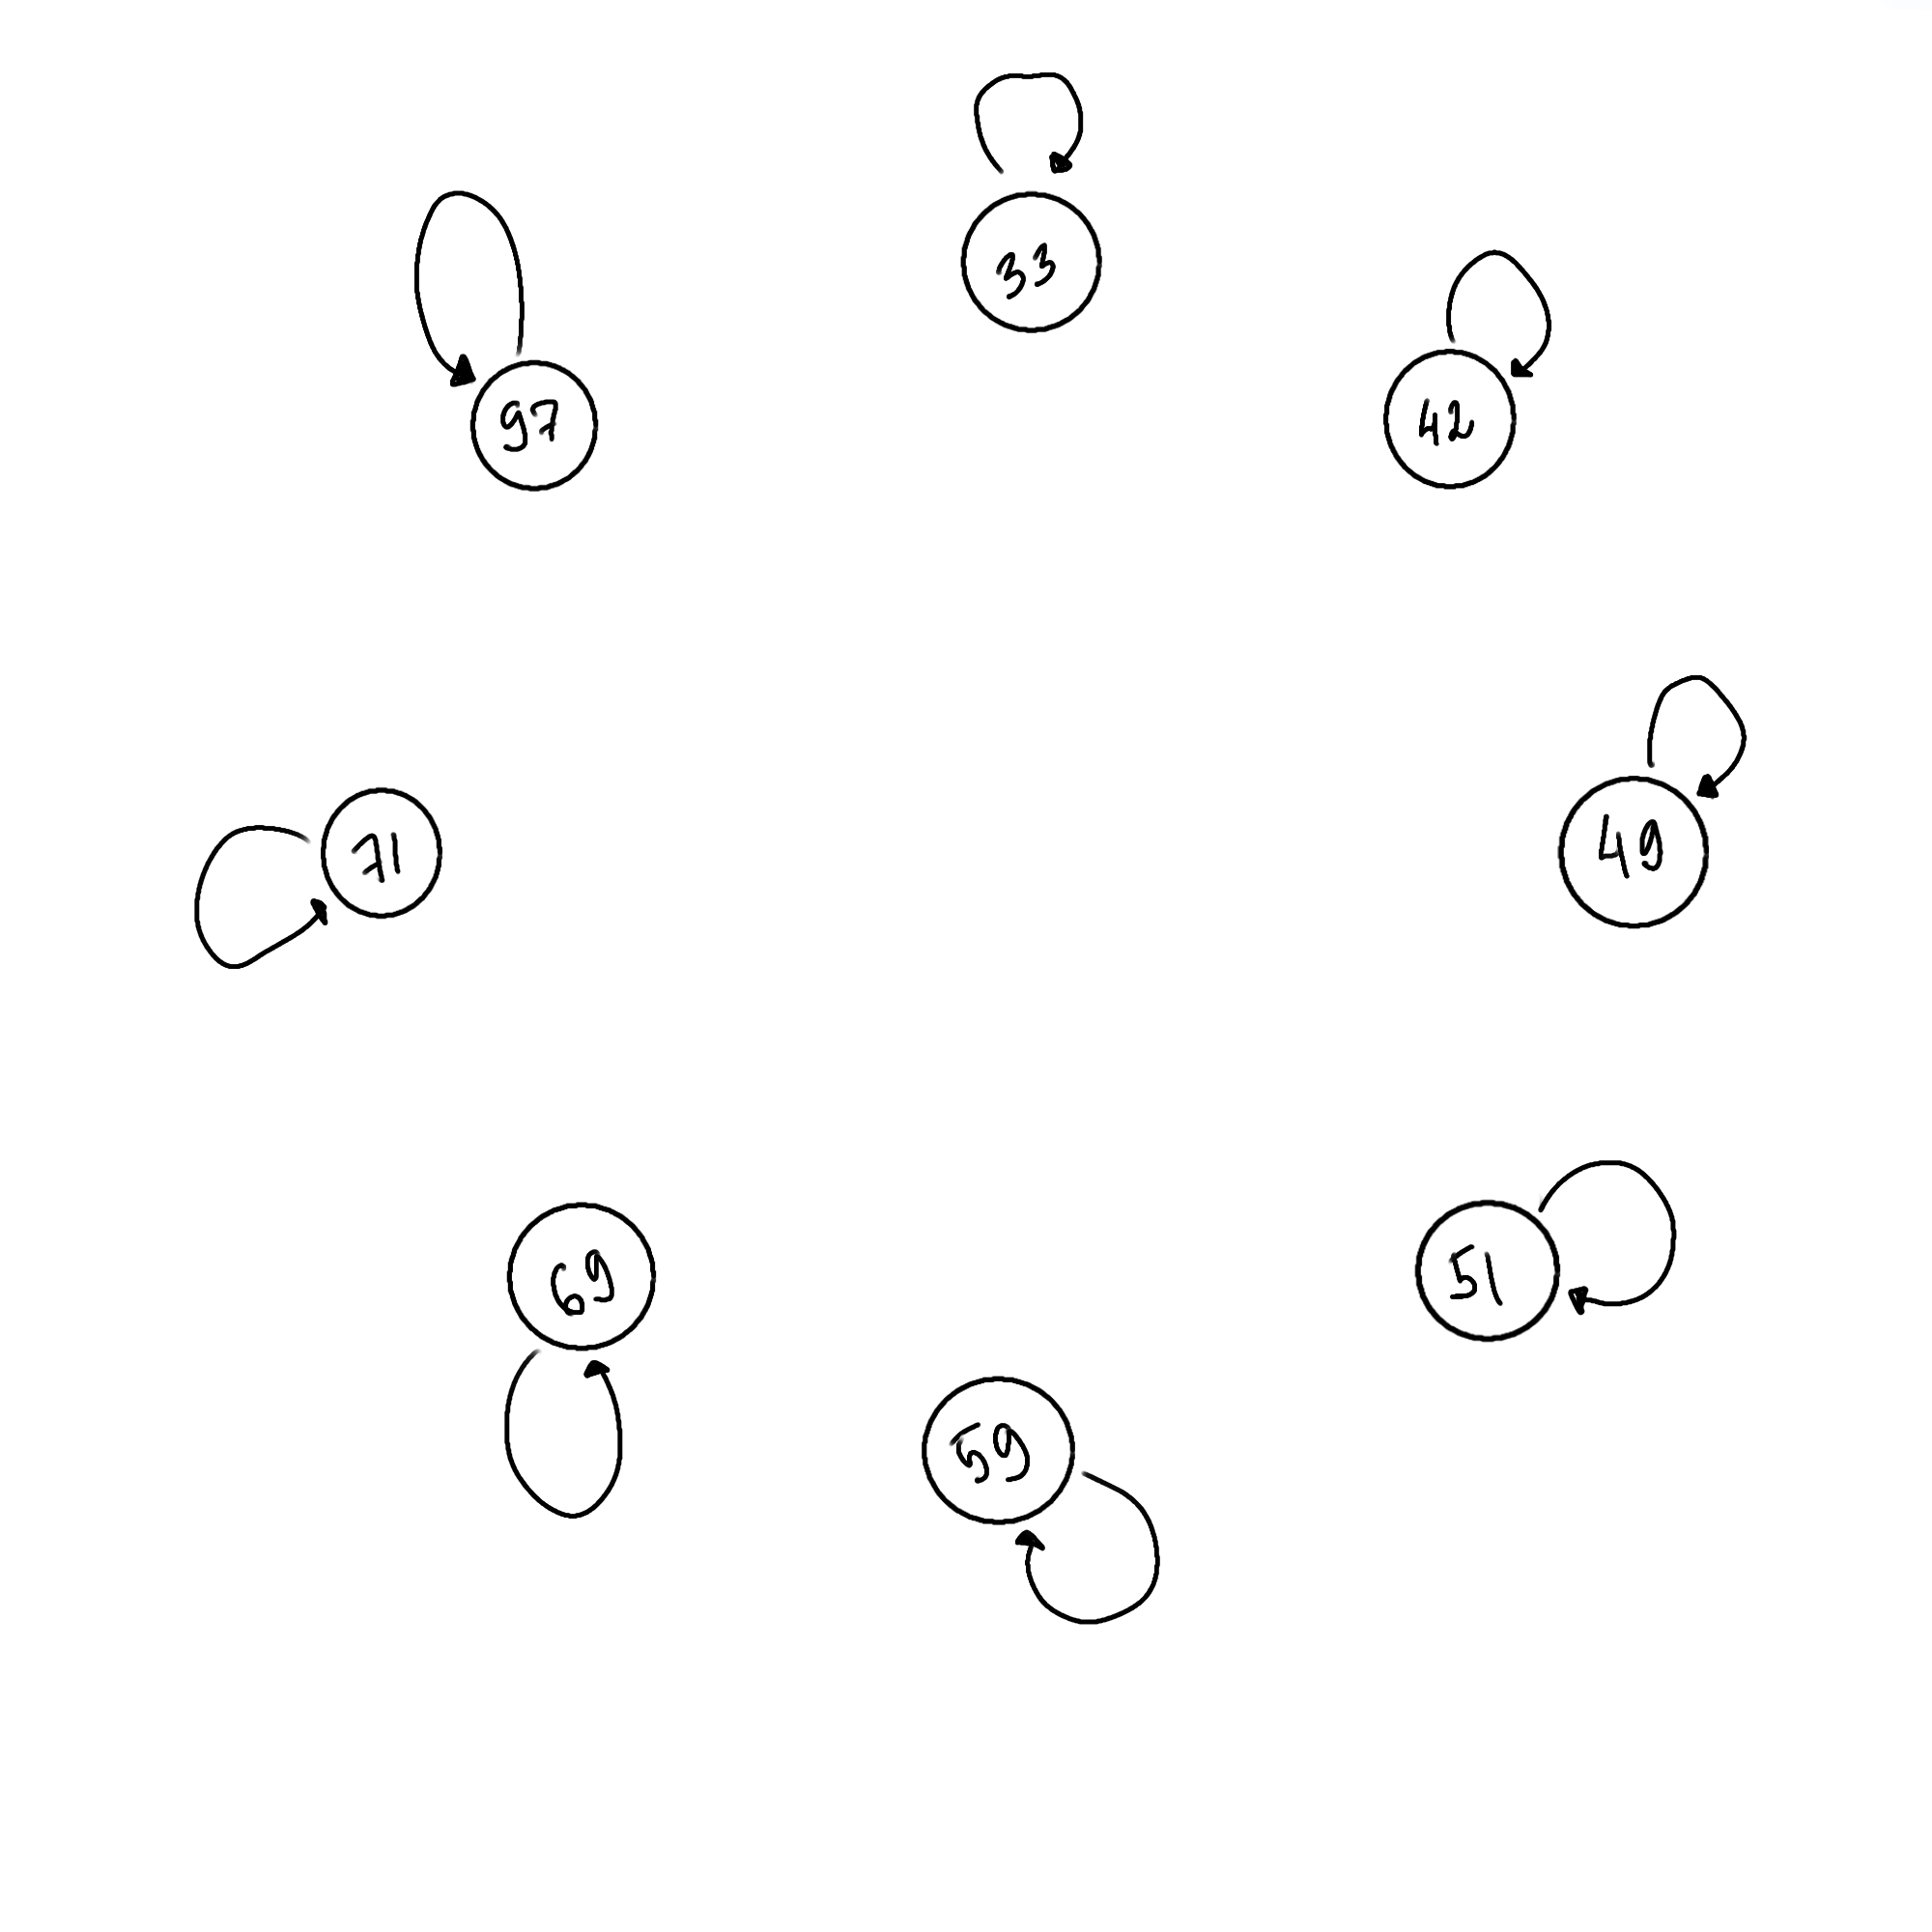
\includegraphics{граф3.png}
\end{proof}

%%%%%%%%%%%%%% ЗАДАНИЕ №3 %%%%%%%%%%%%%%
%% Условие задания №3
\begin{problem}
	Определить, является ли это б.о. отношением эквивалентности, частичного порядка, линейного порядка, строгого порядка.
\end{problem}

%% Решение задания №3
\begin{proof}
	Б. о. является отношением эквиваллентности и частичного порядка, тк рефлексивно, симметрично, антисимметрично и трназитивно.
\end{proof}
%%%%%%%%%%%%%% ЗАДАНИЕ №4 %%%%%%%%%%%%%%
%% Условие задания №4
\begin{problem}
	Для отношений эквивалентности построить классы эквивалентности.
\end{problem}

%% Решение задания №4
\begin{proof}
    \{ 33\}\{ 42\}\{ 49\}\{ 51\}\{ 59\}\{ 69\}\{ 71\}\{ 97\}
\end{proof}
%%%%%%%%%%%%%% ЗАДАНИЕ №5 %%%%%%%%%%%%%%
%% Условие задания №5
\begin{problem}
	Для отношений частичного порядка применить алгоритм топологической сортировки и получить отношение линейного порядка.
\end{problem}

%% Решение задания №5
\begin{proof}
    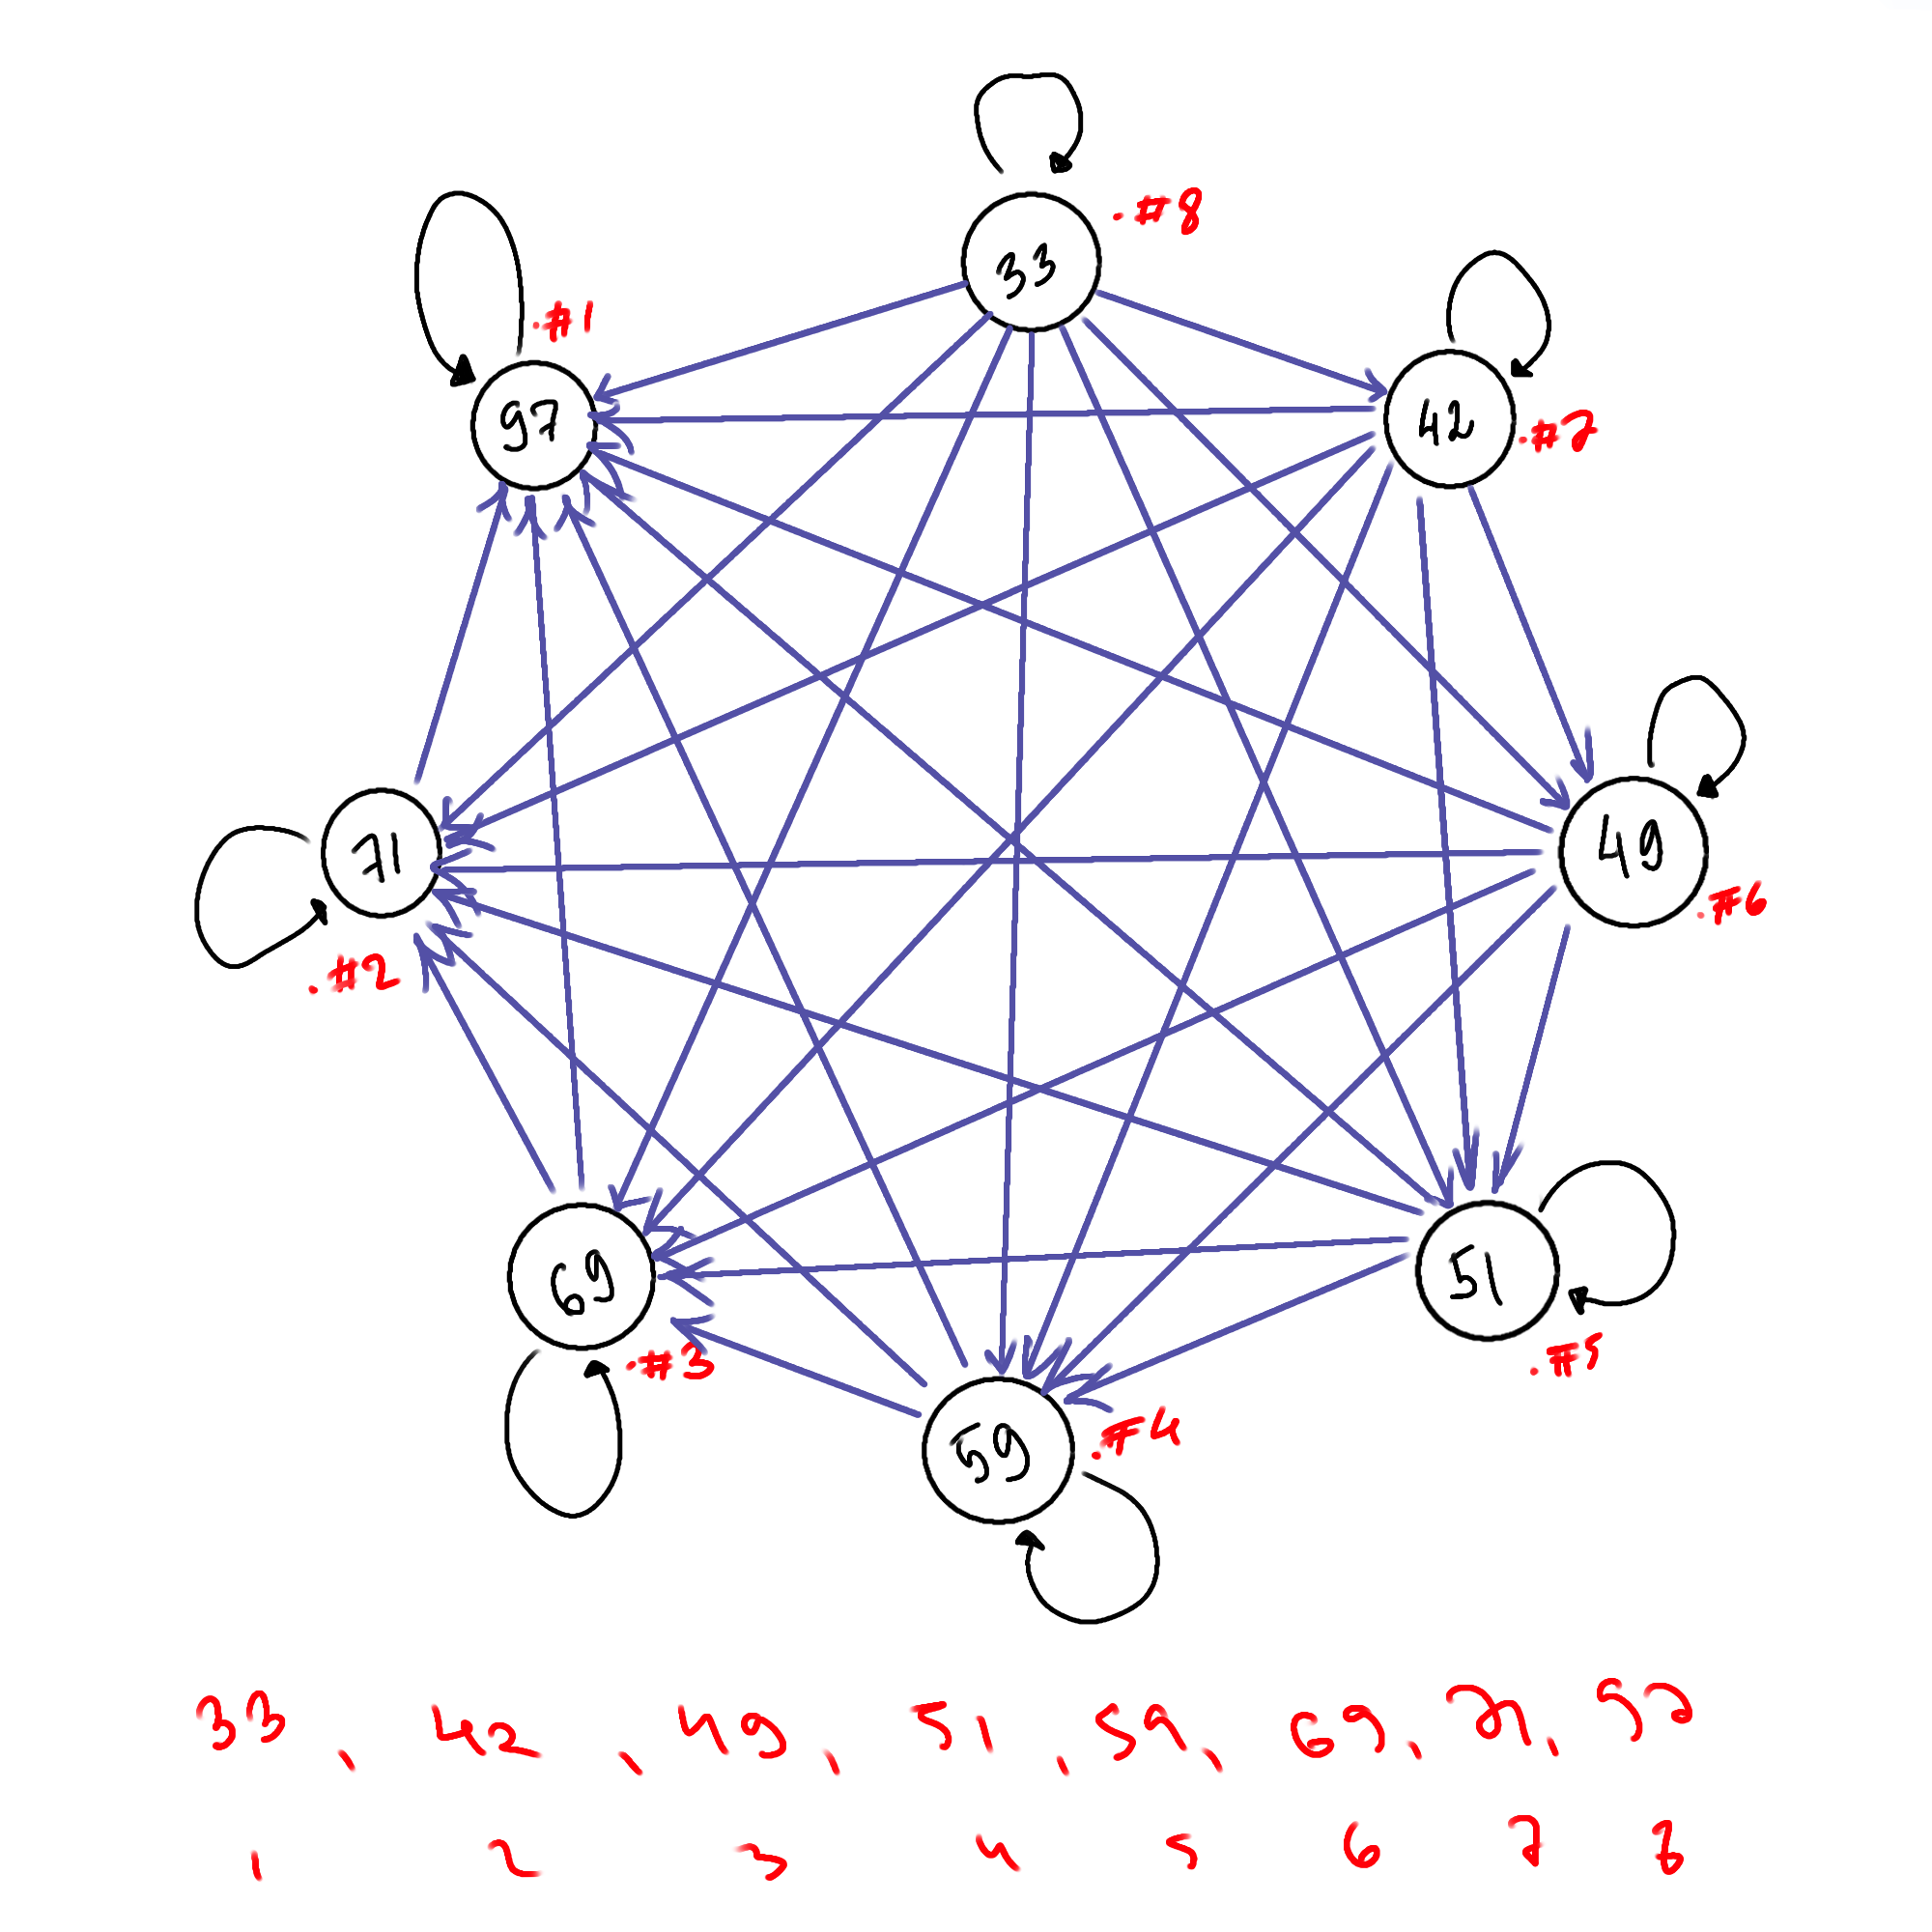
\includegraphics{сортировка2.png}
\end{proof}
%%%%%%%%%%%%%% ЗАДАНИЕ №6 %%%%%%%%%%%%%%
%% Условие задания №6
\begin{problem}
	Для нетранзитивных отношений построить транзитивное замыкание, используя алгоритм Уоршелла.
\end{problem}

%% Решение задания №6
\begin{proof}
Б.о. транзитивно.
\end{proof}
    %%%%%%%%%%%%%% ЗАДАНИЕ №1 %%%%%%%%%%%%%%
%% Условие задания №1
\begin{problem}
    
    М=\{33, 97, 69, 71, 42, 49, 51, 59\}\newline
	Бинарное отношение задано выражением: \newline
   $$ F_{1}(x,y)=1\Leftrightarrow\newline$$
 \newline
 Проверить, является ли бинарное отношение (далее -- б.о.) -- рефлексивным, арефлексивным, симметричным, антисимметричным, асимметричным, транзитивным.
\end{problem}

%% Решение задания №1
\begin{proof}
    Для удобства расположим числа, входящие в мн-во М в порядке возрастания и построим матрицу для данного бинарного отношения:
	$$ \left( \begin{array}{c c c c c c c c } 
 
 1 & 0 & 1 & 1 & 1 & 1 & 1 & 1 \\ 

 0 & 1 & 0 & 0 & 0 & 0 & 0 & 0 \\

 1 & 0 & 1 & 1 & 1 & 1 & 1 & 1 \\ 
 
 1 & 0 & 1 & 1 & 1 & 1 & 1 & 1 \\ 
 
 1 & 0 & 1 & 1 & 1 & 1 & 1 & 1 \\ 
 
 1 & 0 & 1 & 1 & 1 & 1 & 1 & 1 \\ 
 
 1 & 0 & 1 & 1 & 1 & 1 & 1 & 1 \\ 
 
 1 & 0 & 1 & 1 & 1 & 1 & 1 & 1  \end {array} \right) $$
 Б.о. рефлексивно, тк на главной диагонали матрицы все 1.
    \newline
     Б.о. симметрично, тк матрица симметрична относительно главной диагонали.
    \newline
    Б.о. транзитивно, тк при возведении матрицы в квадрат не появляются новые связи.
     \newline

\end{proof}

%%%%%%%%%%%%%% ЗАДАНИЕ №2 %%%%%%%%%%%%%%
%% Условие задания №2
\begin{problem}
	Постройте матрицу и граф этого б.о.
\end{problem}

%% Решение задания №2
\begin{proof}
Перед построением матрицы отсортируем вершины по возрастанию. Таким образом строчке(столбцу) с меньшим порядковым номером соответсвует вершина с меньшим значением, а строчке(столбцу) с большим порядковым номером -- вершина с большим значением.
	$$ \left( \begin{array}{c c c c c c c c } 
 
 1 & 0 & 1 & 1 & 1 & 1 & 1 & 1 \\ 

 0 & 1 & 0 & 0 & 0 & 0 & 0 & 0 \\

 1 & 0 & 1 & 1 & 1 & 1 & 1 & 1 \\ 
 
 1 & 0 & 1 & 1 & 1 & 1 & 1 & 1 \\ 
 
 1 & 0 & 1 & 1 & 1 & 1 & 1 & 1 \\ 
 
 1 & 0 & 1 & 1 & 1 & 1 & 1 & 1 \\ 
 
 1 & 0 & 1 & 1 & 1 & 1 & 1 & 1 \\ 
 
 1 & 0 & 1 & 1 & 1 & 1 & 1 & 1  \end {array} \right) $$
 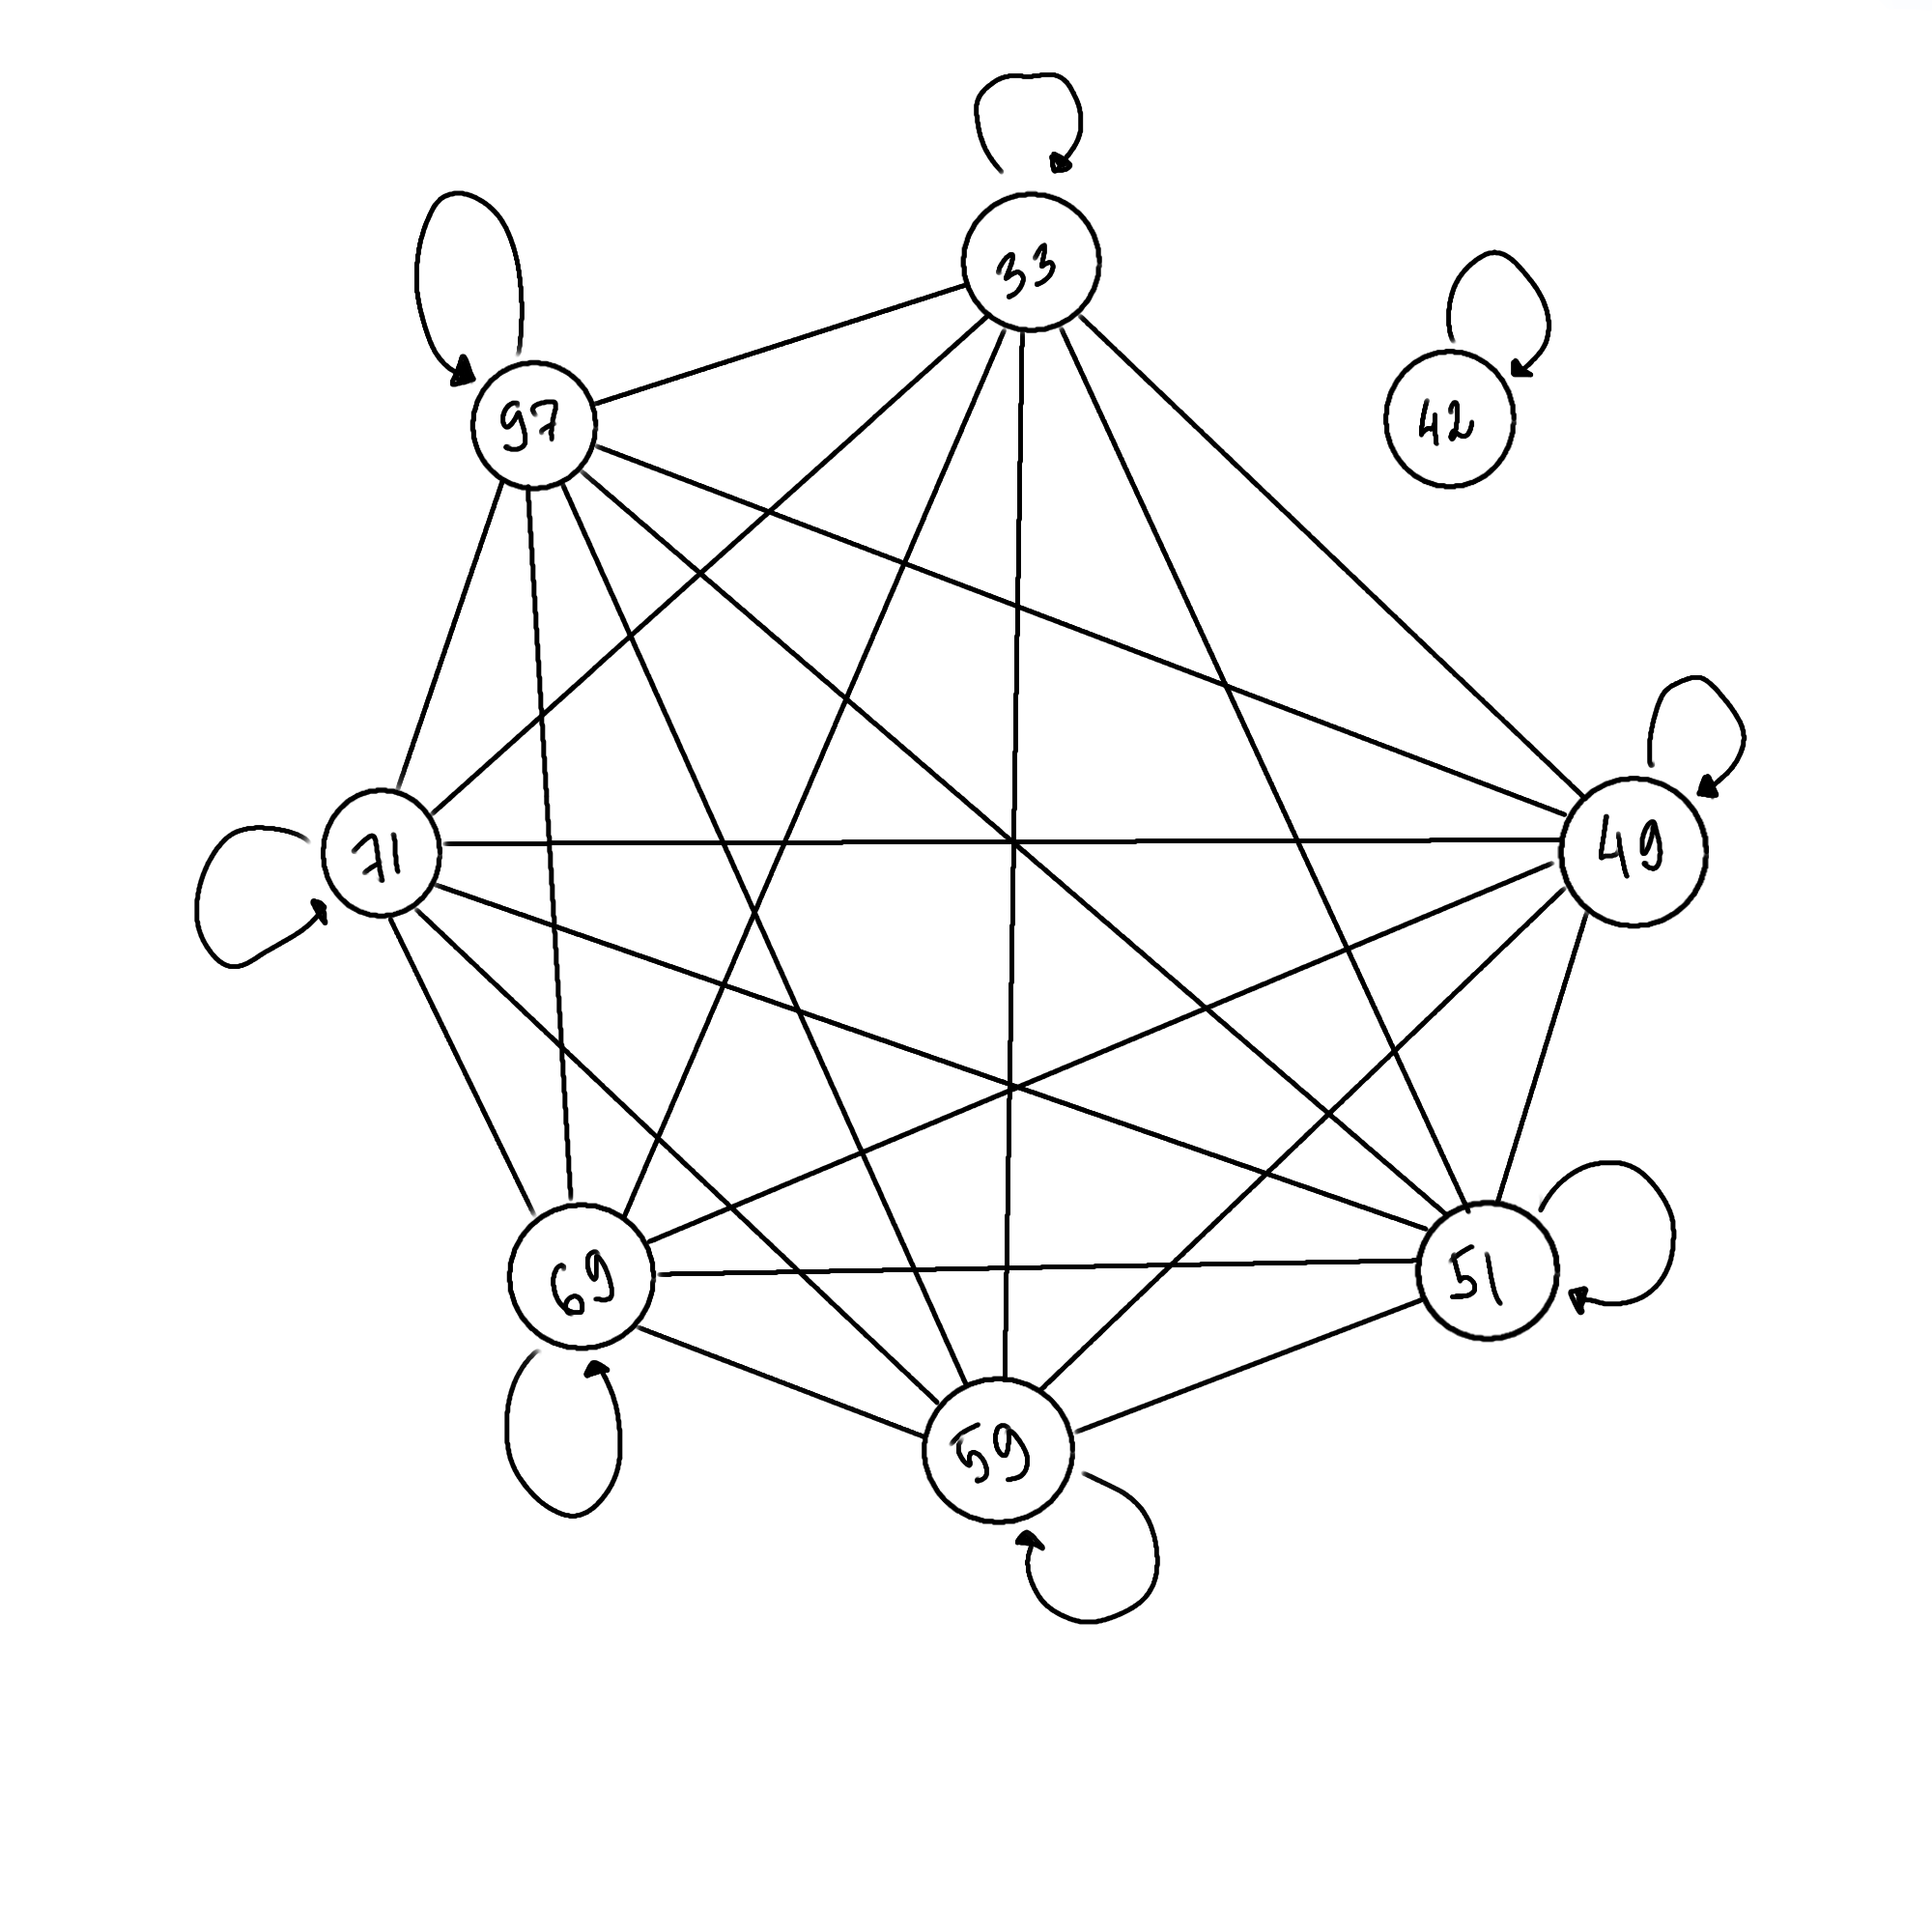
\includegraphics{граф4.png}
\end{proof}

%%%%%%%%%%%%%% ЗАДАНИЕ №3 %%%%%%%%%%%%%%
%% Условие задания №3
\begin{problem}
	Определить, является ли это б.о. отношением эквивалентности, частичного порядка, линейного порядка, строгого порядка.
\end{problem}

%% Решение задания №3
\begin{proof}
	Б. о. является отношением эквиваллентности, тк рефлексивно, симметрично и транзитивно.
\end{proof}
%%%%%%%%%%%%%% ЗАДАНИЕ №4 %%%%%%%%%%%%%%
%% Условие задания №4
\begin{problem}
	Для отношений эквивалентности построить классы эквивалентности.
\end{problem}

%% Решение задания №4
\begin{proof}
\{ 33, 49, 51, 59, 69, 71, 97\}\{ 42\}
\end{proof}
%%%%%%%%%%%%%% ЗАДАНИЕ №5 %%%%%%%%%%%%%%
%% Условие задания №5
\begin{problem}
	Для отношений частичного порядка применить алгоритм топологической сортировки и получить отношение линейного порядка.
\end{problem}

%% Решение задания №5
\begin{proof}
    Б. о. не является отношением частичного порядка.
\end{proof}
%%%%%%%%%%%%%% ЗАДАНИЕ №6 %%%%%%%%%%%%%%
%% Условие задания №6
\begin{problem}
	Для нетранзитивных отношений построить транзитивное замыкание, используя алгоритм Уоршелла.
\end{problem}

%% Решение задания №6
\begin{proof}
Б.о. транзитивно.
\end{proof}
    %%%%%%%%%%%%%% ЗАДАНИЕ №1 %%%%%%%%%%%%%%
%% Условие задания №1
\begin{problem}
    
    М=\{33, 97, 69, 71, 42, 49, 51, 59\}\newline
	Бинарное отношение задано выражением: \newline
   $$ F_{1}(x,y)=1\Leftrightarrow\newline$$
 \newline
 Проверить, является ли бинарное отношение (далее -- б.о.) -- рефлексивным, арефлексивным, симметричным, антисимметричным, асимметричным, транзитивным.
\end{problem}

%% Решение задания №1
\begin{proof}
    Для удобства расположим числа, входящие в мн-во М в порядке возрастания и построим матрицу для данного бинарного отношения:
	$$ \left( \begin{array}{c c c c c c c c } 
 
 1 & 0 & 0 & 0 & 0 & 0 & 0 & 0 \\ 

 0 & 1 & 0 & 0 & 0 & 0 & 0 & 0 \\

 0 & 0 & 1 & 0 & 0 & 0 & 0 & 0 \\
 
 0 & 0 & 0 & 1 & 1 & 0 & 0 & 0 \\
 
 0 & 0 & 0 & 1 & 1 & 0 & 0 & 0 \\
 
 0 & 0 & 0 & 0 & 0 & 1 & 1 & 0 \\
 
 0 & 0 & 0 & 0 & 0 & 1 & 1 & 0 \\
 
 0 & 0 & 0 & 0 & 0 & 0 & 0 & 1  \end {array} \right) $$

 Б.о. рефлексивно, тк на главной диагонали матрицы все 1.
    \newline
     Б.о. симметрично, тк матрица симметрична относительно главной диагонали.
    \newline
    Б.о. транзитивно, тк при возведении матрицы в квадрат не появляются новые связи.
\end{proof}

%%%%%%%%%%%%%% ЗАДАНИЕ №2 %%%%%%%%%%%%%%
%% Условие задания №2
\begin{problem}
	Постройте матрицу и граф этого б.о.
\end{problem}

%% Решение задания №2
\begin{proof}
Перед построением матрицы отсортируем вершины по возрастанию. Таким образом строчке(столбцу) с меньшим порядковым номером соответсвует вершина с меньшим значением, а строчке(столбцу) с большим порядковым номером -- вершина с большим значением.
	$$ \left( \begin{array}{c c c c c c c c } 
 
 1 & 0 & 0 & 0 & 0 & 0 & 0 & 0 \\ 

 0 & 1 & 0 & 0 & 0 & 0 & 0 & 0 \\

 0 & 0 & 1 & 0 & 0 & 0 & 0 & 0 \\
 
 0 & 0 & 0 & 1 & 1 & 0 & 0 & 0 \\
 
 0 & 0 & 0 & 1 & 1 & 0 & 0 & 0 \\
 
 0 & 0 & 0 & 0 & 0 & 1 & 1 & 0 \\
 
 0 & 0 & 0 & 0 & 0 & 1 & 1 & 0 \\
 
 0 & 0 & 0 & 0 & 0 & 0 & 0 & 1  \end {array} \right) $$
 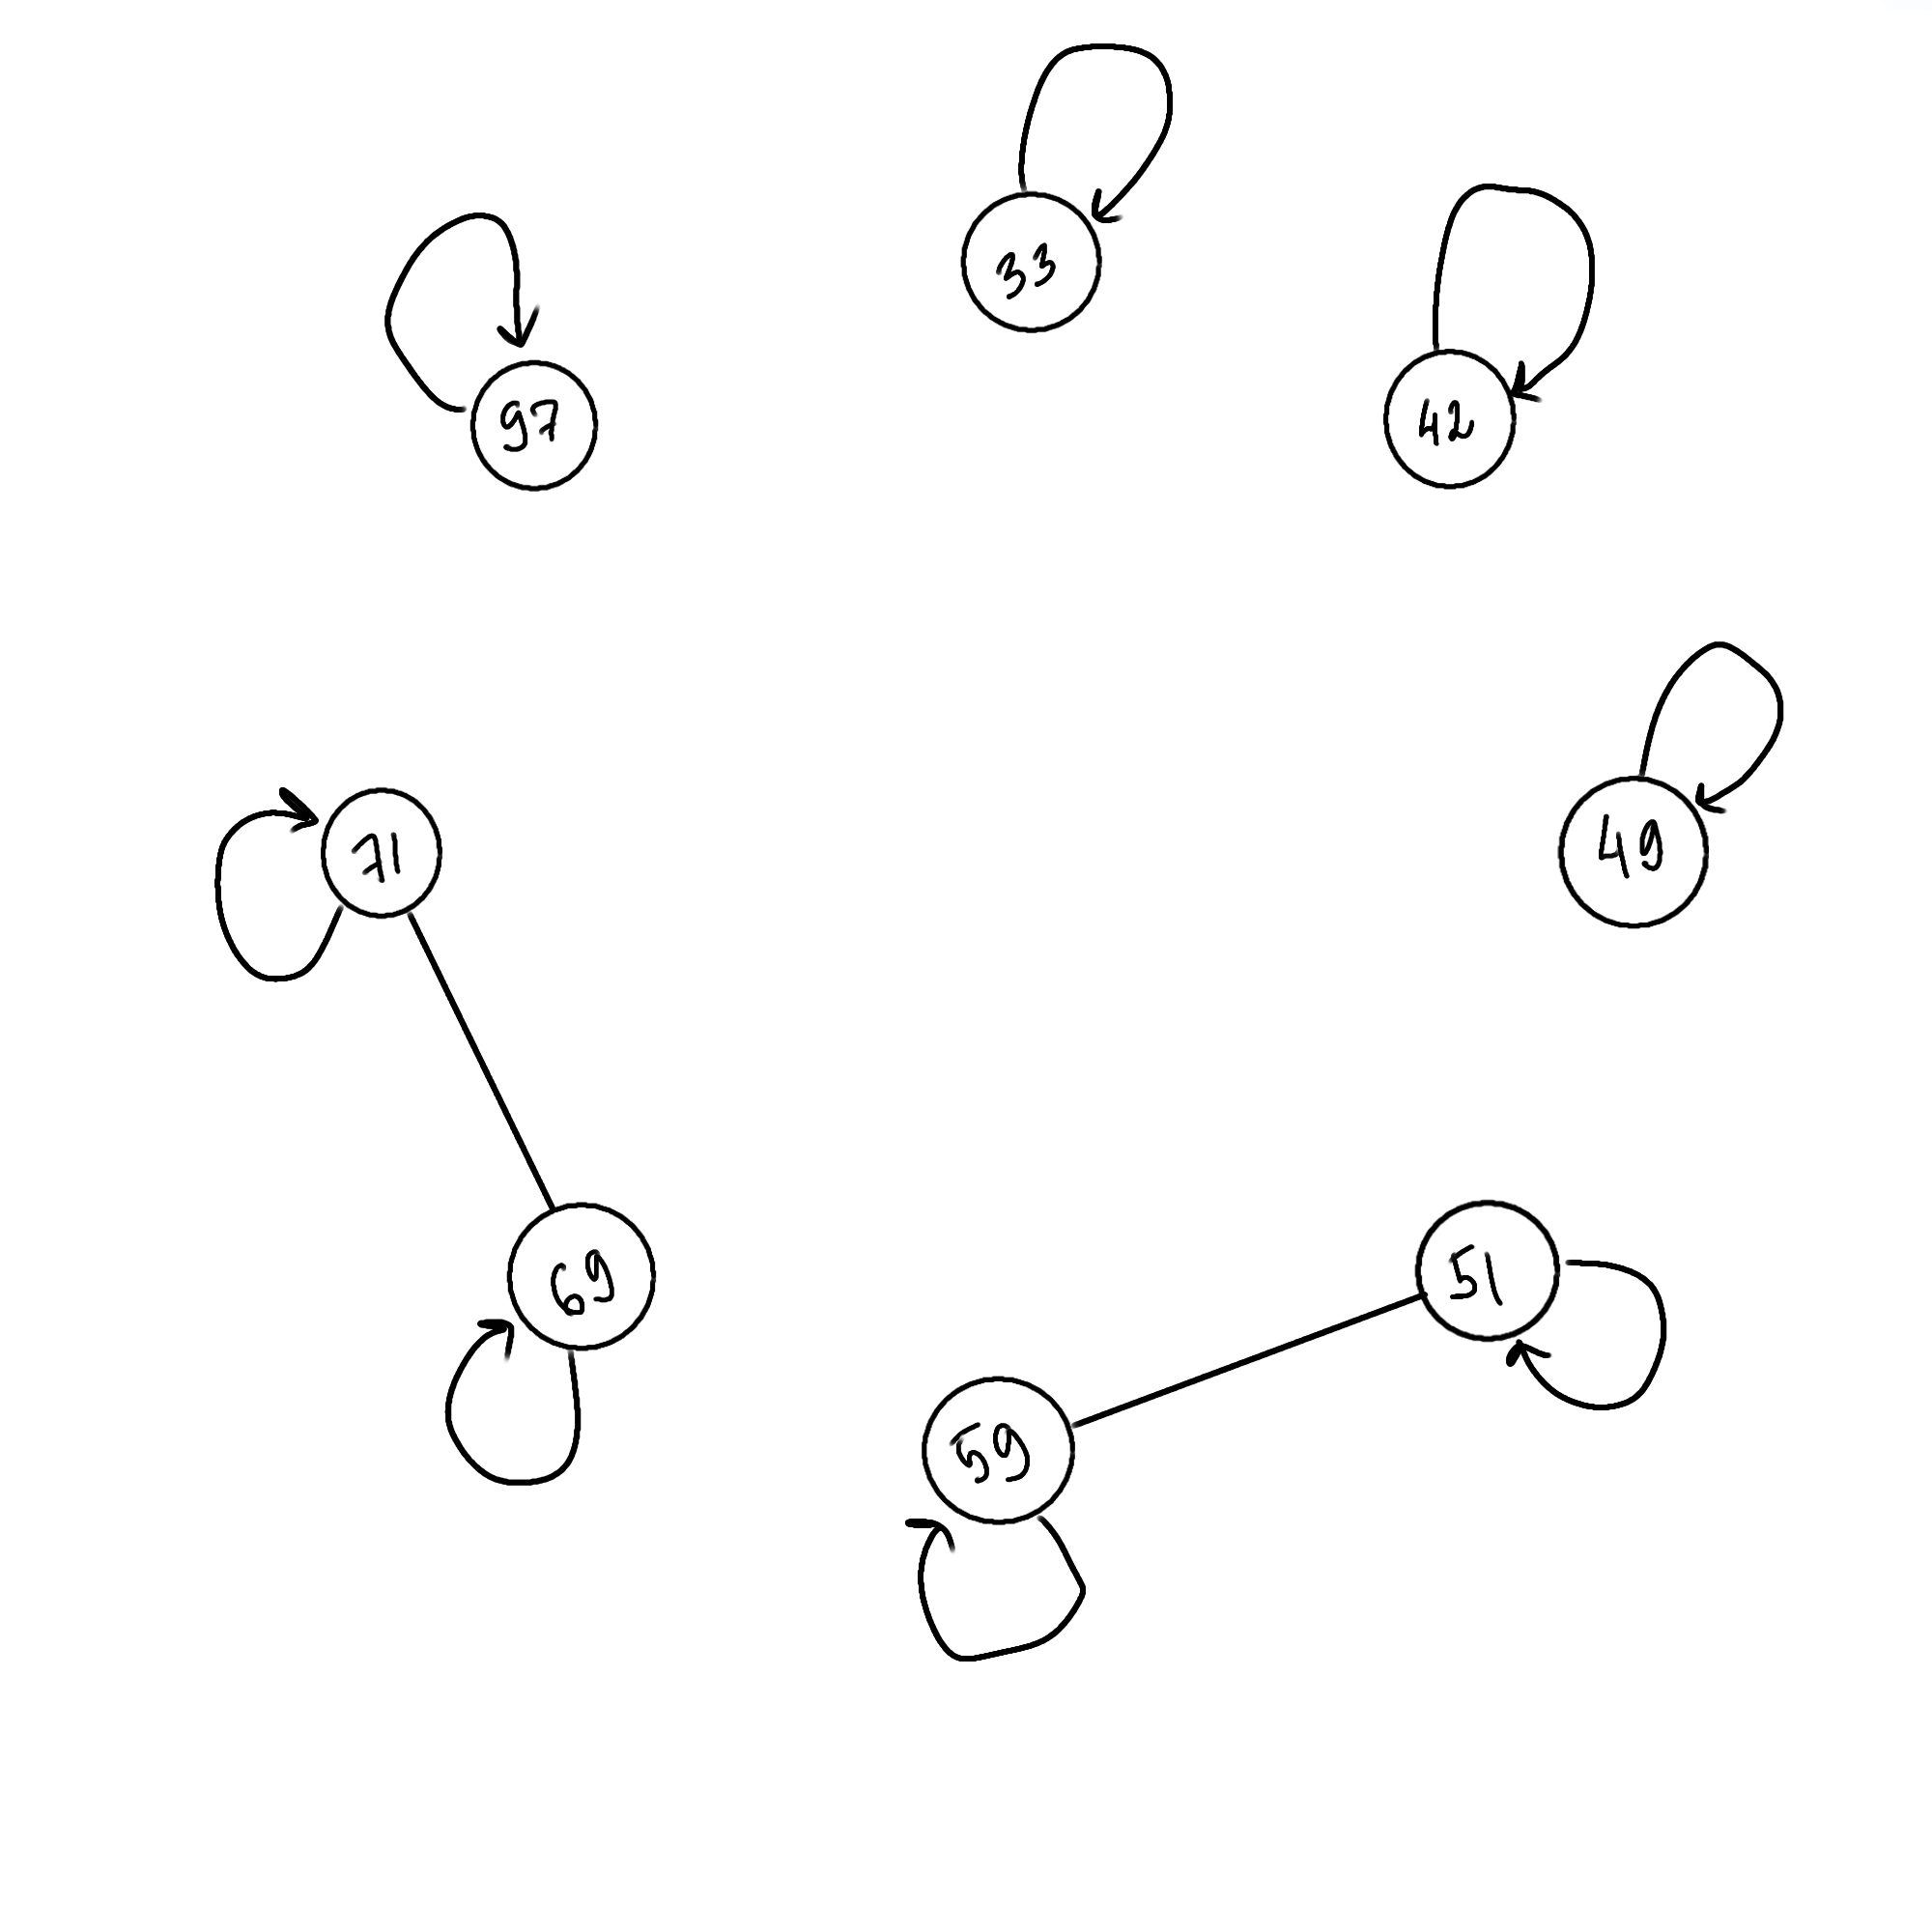
\includegraphics{граф5.png}
\end{proof}

%%%%%%%%%%%%%% ЗАДАНИЕ №3 %%%%%%%%%%%%%%
%% Условие задания №3
\begin{problem}
	Определить, является ли это б.о. отношением эквивалентности, частичного порядка, линейного порядка, строгого порядка.
\end{problem}

%% Решение задания №3
\begin{proof}
	Б. о. является отношением эквиваллентности, тк рефлексивно, симметрично и транзитивно.
\end{proof}
%%%%%%%%%%%%%% ЗАДАНИЕ №4 %%%%%%%%%%%%%%
%% Условие задания №4
\begin{problem}
	Для отношений эквивалентности построить классы эквивалентности.
\end{problem}

%% Решение задания №4
\begin{proof}
\{ 33\}\{ 42\}\{ 49\}\{ 51, 59\}\{ 69\}\{ 71, 97\}
\end{proof}
%%%%%%%%%%%%%% ЗАДАНИЕ №5 %%%%%%%%%%%%%%
%% Условие задания №5
\begin{problem}
	Для отношений частичного порядка применить алгоритм топологической сортировки и получить отношение линейного порядка.
\end{problem}

%% Решение задания №5
\begin{proof}
    Б. о. не является отношением частичного порядка.
\end{proof}
%%%%%%%%%%%%%% ЗАДАНИЕ №6 %%%%%%%%%%%%%%
%% Условие задания №6
\begin{problem}
	Для нетранзитивных отношений построить транзитивное замыкание, используя алгоритм Уоршелла.
\end{problem}

%% Решение задания №6
\begin{proof}
Б.о. транзитивно.
\end{proof}
\end{document}